
\chapter{Sabertooth Motor Driver System}
\label{chap:sabertooth}

RUDRAv4 uses two Dimension Engineering Sabertooth dual regenerative motor drivers.  Each driver controls two brushed DC motors, so two boards support the four-wheel differential-drive base.  The RUDRA design uses packetized serial from the Teensy to the Sabertooths rather than direct PWM from the NUC.

\begin{figure}[h]
\centering
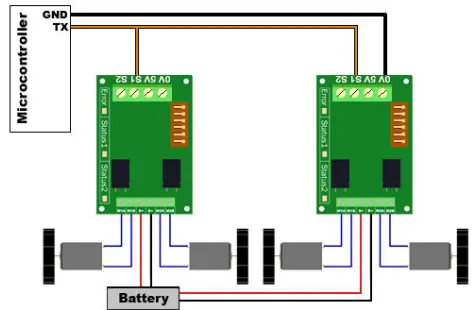
\includegraphics[width=0.92\linewidth]{figures/photos/sabertooth_wiring_article.png}
\caption{Sabertooth motor-driver wiring concept preserved from the RUDRA article assets.}
\end{figure}

\section{Why the Sabertooth is used}
A small H-bridge module can spin a motor on a bench, but RUDRA needs a driver that can tolerate real robot loads, regenerative events, bidirectional drive, and differential steering.  The Sabertooth 2x12 class driver is designed for medium robots and supports multiple control modes, including serial and packetized serial.  In RUDRAv4, packetized serial keeps the wiring simple: one Teensy serial bus can command both motor-controller addresses.

\section{Addressing model}
The current RUDRAv4 firmware contract uses:

\begin{lstlisting}[caption={Sabertooth address contract.}]
Right Sabertooth address: 128
Left  Sabertooth address: 129
Packet serial baud:       9600
Motor command range:      -127 to +127
\end{lstlisting}

The Teensy is the only board that talks packet serial to the Sabertooths.  The NUC sends high-level drive commands to the Teensy; the Teensy converts those commands into Sabertooth packet serial.

\begin{figure}[htbp]
\centering
\resizebox{0.92\linewidth}{!}{%
\begin{tikzpicture}[node distance=8mm and 11mm, every node/.append style={font=\small}]
  \node[rudraBlock,text width=31mm] (nuc) {NUC ROS~2\\\topic{/cmd_vel} or PS2 bridge};
  \node[rudraTopic,text width=32mm,right=of nuc] (packet) {USB serial\\\cmd{D,left,right,enable}};
  \node[rudraBlock,text width=28mm,right=of packet] (teensy) {Teensy~4.1\\base controller};
  \node[rudraHw,text width=25mm,below left=12mm and 2mm of teensy] (leftsab) {Sabertooth\\addr~129};
  \node[rudraHw,text width=25mm,below right=12mm and 2mm of teensy] (rightsab) {Sabertooth\\addr~128};
  \node[rudraHw,text width=25mm,below=of leftsab] (lmotors) {Left-side\\motors};
  \node[rudraHw,text width=25mm,below=of rightsab] (rmotors) {Right-side\\motors};
  \draw[rudraArrow] (nuc) -- (packet);
  \draw[rudraArrow] (packet) -- (teensy);
  \draw[rudraArrow] (teensy) -- node[left,pos=0.45]{\scriptsize Serial1 9600} (leftsab);
  \draw[rudraArrow] (teensy) -- node[right,pos=0.45]{\scriptsize Serial1 9600} (rightsab);
  \draw[rudraArrow] (leftsab) -- (lmotors);
  \draw[rudraArrow] (rightsab) -- (rmotors);
\end{tikzpicture}}
\caption{Command path from ROS to the two Sabertooth motor-driver addresses. The diagram is redrawn in a compact vertical layout to keep all labels legible.}
\end{figure}

\section{DIP switches and packet serial}
The DIP switches define the Sabertooth operating mode and addressing.  Treat the switch position as hardware configuration, not software.  Photograph the final positions and include them in the robot logbook.  The address figure below is retained as a practical wiring reference.

\begin{figure}[h]
\centering
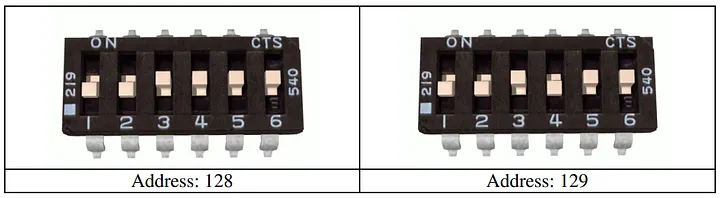
\includegraphics[width=0.75\linewidth]{figures/photos/sabertooth_dip_switch_article.png}
\caption{Sabertooth address setup reference from the original RUDRA material.  Verify against the current Dimension Engineering user guide before changing switch positions.}
\end{figure}

\section{Command mapping}
The RUDRAv4 bridge maps joystick or \topic{/cmd_vel} intent into left and right commands.  At the low level, each command is saturated to the Sabertooth signed command limit:
\begin{equation}
D_L=\mathrm{sat}_{[-127,127]}(k_v v - k_\omega \omega), \qquad
D_R=\mathrm{sat}_{[-127,127]}(k_v v + k_\omega \omega).
\end{equation}

For manual PS2 operation, the current behavior preserves the older RUDRA mixing convention:
\begin{equation}
\mathrm{left}=\mathrm{throttle}-\mathrm{steering}, \qquad
\mathrm{right}=\mathrm{throttle}+\mathrm{steering}.
\end{equation}

In closed-loop operation, those commands become wheel-speed targets; encoder feedback is used to reduce the difference between requested and measured wheel velocity.

\section{Regeneration and battery safety}
A regenerative driver can push energy back toward the battery during deceleration or when the robot is driven by external forces.  This is useful but it makes power wiring important.  The motor battery must remain connected when the Sabertooths are powered, and the emergency stop should remove motive power in a controlled manner.  Do not test motors with a weak supply, floating battery connection, or undersized bench supply that cannot tolerate regen.

\section{Motor bring-up procedure}
\begin{enumerate}
  \item Disconnect or lift all wheels.
  \item Confirm motor battery polarity and Sabertooth power wiring.
  \item Confirm each Sabertooth address with a small command.
  \item Send zero command and verify all motors stop.
  \item Send low positive left and right commands independently.
  \item Fix sign errors in firmware mapping, not by swapping random wires after the robot is assembled.
  \item Confirm the command timeout stops all motors when the NUC serial bridge is killed.
  \item Only then place the robot on the floor at low speed.
\end{enumerate}

\begin{safetybox}{Single owner of the Teensy serial port}
Never run \pkg{ps2_uno_to_teensy} and \pkg{cmd_vel_to_teensy} at the same time.  Both attempt to own the Teensy USB serial device, and both can generate motor commands.  Pick one drive bridge per test.
\end{safetybox}
